% The 12pt option is required by the 2001/02 thesis regulations
% Last update 15th August 2007: new Abstract format and Copyright Statement

% Replace MSc with PhD for PhD theses
% Remove the twoside option for single-sided printing
\documentclass[12pt,PhD,twoside]{muthesis}

%These are the citation styles.
\usepackage[backend=biber,style=nature,citestyle=nature]{biblatex}
\usepackage{graphicx}
\addbibresource{references.bib}
\graphicspath{ {images/} }

\begin{document}
\title{Investigating the Recognition and Interactions of Non-Polar $\alpha$ Helices in Biology.}
\author{James Baker}
% Faculty of Life Sciences people should comment the next line out
%\school{Mathematics}
\faculty{Life Sciences}
\def\wordcount{xxxxx}

% Uncomment the line below to suppress the `List of Tables' page (optional)
%\tablespagefalse

% Uncomment the line below to suppress the `List of Figures' page (optional)
%\figurespagefalse

% Uncomment the line below to use a customised Declaration statement
%\def\declaration{All the work in this thesis has been sourced from Google.}

\beforeabstract

Transmembrane $\alpha$ helix containing proteins make up around a quarter of all proteins, as well as two thirds of drug targets, and contain some of the most critical proteins required for life as we know it. Yet they are fundamentally difficult to study experimentally due to the very features that make them so biologically influential: their hydrophobic transmembrane helices. What is missing in the current literature is a complex, nuanced understanding of this helix composition. Currently it is known that the properties of transmembrane protein $\alpha$-helices underpin membrane protein insertion mechanisms and furthermore can be used to predict presence of function in the transmembrane helix itself. By leveraging large datasets of transmembrane proteins, this thesis is focussed on characterising features of $\alpha$ helices en masse, particularly regarding their topology, membrane-protein interactions, and intra-membrane protein interactions.

Herein we expand on the core understanding of the biophysicochemical properties of these helices. We find evidence of a universal, ``negative-not-inside'' rule that complements the famous ``positive-inside rule'' as well as intramembrane leucine propensity for the inner leaflet.

\afterabstract

\prefacesection{Acknowledgements}
So long! And thanks for all the fish.

\prefacesection{List of publications}

\afterpreface % DO NOT DELETE. BAD THINGS HAPPEN.

\chapter{Introduction}
\section{The importance of membranes and transmembrane proteins.}
The compartmentalisation of cellular biochemistry is arguably one of the most significant events to have happened in the evolution, and is certainly one of the fundamental prerequisites for life\cite{Koshland2002}.

Transmembrane Proteins (TMPs) underpin almost every biological process directly, or indirectly, from photosynthesis to respiration. Integral TMPs are encoded by around 30\% of the genes in the human genome which reflects their biological importance \cite{Almen2009}.

In the 1990s and early 2000s the Transmembrane Helix (TMH) was a rather simple topological story. TMPs were thought to contain membrane spanning bundles of non-polar α-helices, with each TMH having a consistent orientation of being perpendicular to the membrane surface. Although this is broadly true, hundreds of high quality membrane structures have elucidated that TMHs can adopt a plethora of lengths and orientations within the membrane. TMHs are capable of partial spanning of the membrane, spanning using oblique angles, and even lying flat on the membrane surface \cite{VonHeijne2006, Elofsson2007}.

\begin{figure}[h]
\centering
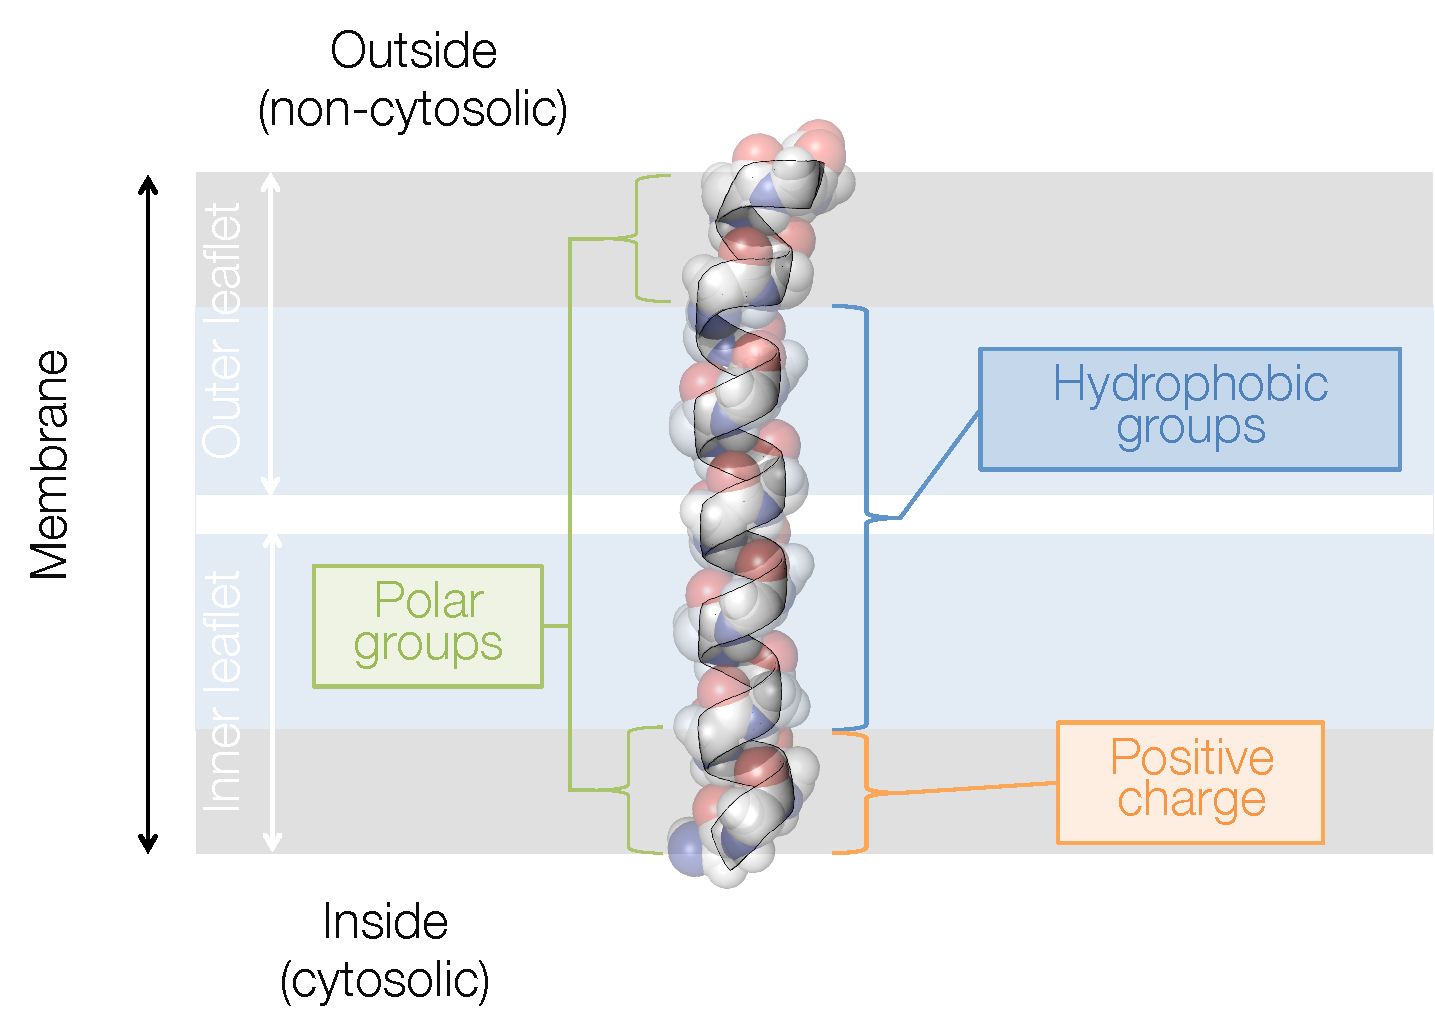
\includegraphics[width=1\textwidth]{Helix_anatomy}
\caption{\textbf{Cartoons of helices in the membrane.} (A) A cartoon showing the general components of the membrane and TMH. Dark grey areas denote the area composed typically or polar or charged amino acid groups. These areas are often described as flanking regions, and are often in contact with the aqueous interface of the membrane. The curved black lines represent the residue chain outside of the membrane. The helix core is mostly composed of hydrophobic groups and is illustrated here in dark orange. More recently the hydrophobic group region has been associated with cell localisation and a broad range of biochemical functions \cite{Junne2010, Wong2012}. Note that the definition of an α-helix is not entirely clear; how far the helix rises into the water-interface region to qualify as a TMH for example \cite{VonHeijne2006}. (B) A cartoon depicting various problematic, yet biologically observed topologies and lengths that the alpha helices can adopt. From left to right: a typical and traditional TMH, an exceptionally long TMH, a TMH that lies flat in the interface region, a kinked helix that enters and exits the bilayer on the same leaflet, a TMH that is not long enough to span the entire membrane. Note that these exceptional formations present a challenge for topology predictions of the loop regions.}
\end{figure}

Because of the experimental hinderence, the story of transmembrane proteins has been relatively slow to emerge. In the 1990s and early 2000s the story was seemingly uncomplicated. There were membrane-spanning bundles of non-polar α-helices of roughly 20 residues length, with a consistent orientation of being perpendicular to the membrane surface. Since the mid-2000s the elucidation of many more intramembrane helix structures implied a far richer variety of transmembrane helices existed than previously thought, with a range of orientations and intra-membrane biophysical variations.

The language used to describe TMHs varies somewhat across the literature, primarily due to a changing understanding of TMH general structure and relevance to function over the last 15 years or so. There is a general composition of a TMH despite specific protein and membrane constraints \cite{Sharpe2010}.

More recently, the insertion and formation of the unusually orientated TMHs and of the more traditional TMHs have been shown to be underpinned by complex thermodynamic equilibria \cite{Cymer2014}. TMHs have been identified as regulators of protein quality control and trafficking mechanisms, shifting the idea away from TMHs broadly simply functioning as anchors \cite{Hessa2011}. The story is not as simple as originally thought. There is a contingency in the field of biological membranes that despite progress over the last decade, there is a lack of information regarding their structure, assembly, and the behaviour of TMHs in the lipid bilayer; the native biological environment of TMHs \cite{Ladokhin2015, Cymer2014}.

Properties that can be analysed by bioinformatics, the sequence complexity and hydrophobicity, of the TMH have been used to predict the role of the TMH as either functional or structural, and as a discrete cluster from other SCOP annotated helices \cite{Wong2012}. Those findings demonstrated that sequence of the TMH holds valuable information regarding biological roles, and forms the basis of our interest in the link between the polarity of a helix and functional activity beyond structural anchorage.

\section{The ``anatomy'' of transmembrane helices}
%This paragraph should certainly be changed to the updated one from the manuscript.
A study by Baeza et al. from 2013 \cite{Baeza-Delgado2013} looked at TMHs in 170 integral membrane proteins from a manually maintained database of experimentally confirmed TMPs; MPTopo \cite{Jayasinghe2001}. The group examined the distribution of residues along the TMHs. As expected, half of the natural amino acids are equally distributed along Transmembrane (TM) helices whereas aromatic, polar, and charged amino acids along with proline are biasedly near the flanks of the TM helices \cite{Baeza-Delgado2013}. Transitions between the different types of amino acid at the ends of the hydrophobic core occur in a more defined region on the cytosolic side than at the extra cytosolic face. This is probably reflecting the different lipid composition of both leaflets of biological membranes \cite{Baeza-Delgado2013}. A larger study using 1192 human and 1119 yeast predicted TMHs that were not structurally validated further explored the difference in TMH and leaflet structure by exploiting the evolutionarily conserved sequence differences between the TMH in the inner and outer leaflets \cite{Sharpe2010}. TMHs from vertebrates and invertebrates were found to be reasonably similar compositionally. The differences in consensus TMH structure implies that there are general differences between the membranes of the golgi and ER. The abundance of serines in the region following the lumenal end of golgi TMDs probably reflects the fact that this part of many golgi enzymes forms a flexible linker that tethers the catalytic domain to the membrane \cite{Sharpe2010}.

\section{The ``Positive-Inside rule''.}
Two publications by von Heijne coined the ``Positive-Inside rule'' demonstrated the practical value of positively charged residue sequence clustering in topology prediction of transmembrane helices in bacteria \cite{VonHeijne1989,VonHeijne1992}. It was clearly defined and shown that positively charged residues more commonly were found on the ``inside'' of the cytoplasm rather than the periplasm. More recently still large scale sequence analysis of transmembrane helices from different organelle membrane surfaces in eukaryotic proteomes, show the clustering of positive charge being cytosolic \cite{Sharpe2010, Baeza-Delgado2013}.

As the idea of positive residues inside the cytoplasm emerged, so did the idea of negative residues working in concert with TMH orientation. It was shown that removing a single lysine residue reversed the topology of a model Escherichia coli protein, whereas much higher numbers of negatively charged residues are needed to reverse topology \cite{Nilsson1990}. One would also expect to see a skew in negatively charged distribution if a cooperation between oppositely charged residues orientated a TMH, however there is no conclusive evidence in the literature for an opposing negatively charged skew \cite{Granseth2005, Nilsson2005, Sharpe2010, Baeza-Delgado2013}. However, in {\it E. coli} negative residues do experience electrical pulling forces when travelling through the SecYEG translocon indicating that negative charges are biologically relevant \cite{Ismail2015}.

\chapter{The ``negative-not-inside rule''}
\chaptermark{Shortened chapter header}

\chapter{Tail-anchored protein discovery}

\chapter{The good \& the bad helices}

\chapter{Conclusions}

\printbibliography[title={Bibliography}]

% Comment the following THREE lines if you do NOT have an Appendix
\appendix
\chapter{Big tables}
.........

\end{document}
